\chapter{Deployment and Testing}
\label{ch:deployment-and-testing}
As mentioned in Section~\ref{ch:design-and-impl}, aiVLE 2.0, especially aiVLE Worker and aiVLE Grader, is designed to be highly scalable and easy to deploy. However, just like any distributed systems, being able to run the individual components on a single machine is one thing, having all the components cooperate on separate machines to achieve actual distribution is another. Thus, to pave way for production deployment in the next academic year, and to demonstrate the actual performance of such a distributed system, we performed a complete deployment using several SoC cluster nodes\footnote{Special thanks to the SoC compute cluster admins and Dr. Narayan for their help in securing these very powerful GPU nodes as shown later in Section~\ref{ss:deployment-environment}.} and did several experiments/benchmarks on the system.

There will be three sections covering both the deployment and tests this chapter: Section~\ref{s:deployment} describes the deployment environment, deployment steps and issues we encountered before making the system fully functional on SoC compute cluster. Section~\ref{s:load-balance-exp} describes the methodology and findings of load balancing among \textbf{multiple} worker nodes. Section~\ref{s:concurrency-exp} describes the methodology and findings of running evaluation jobs concurrently on a \textbf{single} worker node.

\section{Deployment}
\label{s:deployment}
Note that this deployment happened during the winter break (November 2021 to January 2022). Therefore some later updates to the aiVLE Web and Worker are not included during this deployment (most notably, the resource-sensitive load balancing). However, this does not affect the later mentioned test results as the experiments are designed to have no system overloading (see Section \ref{sss:choice-of-params}).

In specific, the exact versions used are (Git commit hash with GitHub link):
\begin{itemize}
    \item aiVLE Web: \href{https://github.com/edu-ai/aivle-web/commit/b346a68e30aa05656ae2e6cc106414bcba5430fd}{b346a68e30aa05656ae2e6cc106414bcba5430fd}
    \item aiVLE Worker: \href{https://github.com/edu-ai/aivle-worker/commit/647d767a72acf6c5f5ded533d77141ca91f4ef9d}{647d767a72acf6c5f5ded533d77141ca91f4ef9d}
\end{itemize}

\subsection{Environment}
\label{ss:deployment-environment}
aiVLE Worker is deployed on SoC compute cluster \texttt{xgpg0, xgpg1, xgpg2} with the following configuration:
\begin{itemize}
    \item Operating System (Code~\ref{code:deployment-os}): Ubuntu 20.04 LTS with Linux kernel version 5.4.0
    \item GPU (Code~\ref{code:deployment-gpu}): NVIDIA A100-PCI, Driver 495.29, CUDA 11.5
    \item CPU: 2x AMD Epyc 7352, in total 48 cores/96 threads, base clock 2.3GHz
    \item RAM: 256GiB DDR4
\end{itemize}

\begin{code}
\begin{minted}[frame=lines,framesep=2mm,baselinestretch=1.2,bgcolor=LightGray,fontsize=\footnotesize,linenos]{shell}
> cat /proc/version
Linux version 5.4.0-91-generic (buildd@lcy01-amd64-017) 
(gcc version 9.3.0 (Ubuntu 9.3.0-17ubuntu1~20.04)) #102-Ubuntu SMP Fri Nov 5 16:31:28 UTC 2021
\end{minted}
\captionof{listing}{Deployment Environment - Operating System}
\label{code:deployment-os}
\end{code}

\begin{code}
\begin{minted}[frame=lines,framesep=2mm,baselinestretch=1.2,bgcolor=LightGray,fontsize=\footnotesize,linenos]{shell}
> nvidia-smi 
Sat Jan  1 13:32:49 2022       
+-----------------------------------------------------------------------------+
| NVIDIA-SMI 495.29.05    Driver Version: 495.29.05    CUDA Version: 11.5     |
|-------------------------------+----------------------+----------------------+
| GPU  Name        Persistence-M| Bus-Id        Disp.A | Volatile Uncorr. ECC |
| Fan  Temp  Perf  Pwr:Usage/Cap|         Memory-Usage | GPU-Util  Compute M. |
|                               |                      |               MIG M. |
|===============================+======================+======================|
|   0  NVIDIA A100-PCI...  On   | 00000000:01:00.0 Off |                    0 |
| N/A   49C    P0    36W / 250W |      0MiB / 40536MiB |      0%      Default |
|                               |                      |             Disabled |
+-------------------------------+----------------------+----------------------+
\end{minted}
\captionof{listing}{Deployment Environment - GPU}
\label{code:deployment-gpu}
\end{code}

aiVLE Web is deployed on a \href{https://linode.com/}{Linode} Nanode 1GB VPS (virtual private server) with 1 virtual CPU core and 1 GiB of RAM.

\subsection{Limitations}
\label{ss:deployment-limitations}
There is one additional problem with distributed systems that we did not mention in the introductory paragraph of this chapter: even if the system works on a few machines, it does not necessarily mean the system will work or scale well to dozens or even hundreds of machines. While we design the system to be highly scalable, and the underlying technologies (i.e., Celery as Python library and RabbitMQ as message queue broker) have proven to be effective on hundreds of machines, we are never certain until we actually scale the system to that many nodes and put it under pressure.

Unfortunately, for the time being, we are unable to materialize such a large-scale experiment: SoC compute cluster does not have that many GPU nodes available (for a final year project at least), nor did we have a demanding enough task to put the system at such a scale under considerable pressure. In fact, on the \texttt{xgpg*} nodes used for this experiment, every evaluation takes $\sim$10 seconds to finish, which is too short for even tens of worker nodes: for the evaluation subsystem to be stressed, we at least need to keep the task queue ``filled''. In other words, the rate of submitting new jobs into the task queue should be much greater than the rate of workers finishing jobs. However, with each job only taking $\sim$10 seconds, suppose we have 50 workers, our rate of consumption would be $50/10=5$ jobs per second (every 10 seconds we can process 50 jobs). If we assume each submission to be $\sim$20MiB\footnote{Many deep learning models are much larger, so we are having a relatively conservative estimation here}, it would require at least 100MiB per second of network throughput, which is already approaching the limit of Gigabit Ethernet available on most machines.

Therefore, with our current resources, it is nearly impossible to properly test the scalability potential of aiVLE 2.0. However, this does not mean that our experiments are useless! Quite the contrary, our experiment setup is on par with the resources available to CS4246 teaching team, and we expect aiVLE 2.0 to have a much higher utilization rate of computational power - as a result, process submissions with smaller delays.

In short, we are cautiously optimistic about the scalability of aiVLE 2.0 as we do not yet have experiment data to support it, but we are confident that it can support CS4246 teaching much more effectively from the experiment results as shown in Section~\ref{s:load-balance-exp} and Section~\ref{s:concurrency-exp}.

\subsection{Steps}
To simulate the production deployment process, we scrapped existing setups and started everything afresh. The following steps are sufficient for any deployment from the ground up:

\begin{enumerate}
    \item Prepare the message queue broker: either by installing \href{https://www.rabbitmq.com/}{RabbitMQ} or using cloud message queue provider such as \href{https://www.cloudamqp.com/}{CloudAMQP}. In our case, we installed RabbitMQ on the same VPS with aiVLE Web.
    \item Install and start aiVLE Web on the VPS.  The aiVLE Web ``readme'' (\href{https://github.com/edu-ai/aivle-web#readme}{https://github.com/edu-ai/aivle-web\#readme}) is the definitive guide on this process.
    \item Setup the users, courses, tasks in aiVLE Web via its RESTful API or Django admin panel.
    \item Prepare the worker nodes with necessary dependencies (i.e., Firejail, Pip, Virtualenv, CUDA drivers). In our case, we requested the cluster admins to install Firejail as all other dependencies are already available.
    \item Install and start aiVLE Worker on the worker nodes. aiVLE Worker ``readme'' (\href{https://github.com/edu-ai/aivle-worker#readme}{https://github.com/edu-ai/aivle-worker\#readme}) describes this process in detail.
\end{enumerate}

\subsection{Issues and Solutions}
There are some issues we found during the deployment process. None of which is critical in a sense that we eventually found workarounds without modifying any existing codebase or design. But we think it is nonetheless useful to point them out here as potential users of this system is likely to encounter some of them as well.

\subsubsection{Switching broker from RabbitMQ to AWS SQS}
If the worker node resides behind a firewall that restricts access to certain ports (especially under a whitelist policy where only selected ports are available), then you are likely to find RabbitMQ unusable - its underlying protocol, Advanced Message Queuing Protocol (AMQP), uses port 5671/5672 by default. There are three possible solutions:
\begin{enumerate}
    \item Change RabbitMQ port to one that is allowed by the worker node firewall. Do note that AMQP is not based on HTTP/HTTPS, so when change the port to 80/443 you need to ensure that not only the broker server has those ports available, but also the worker node firewall DOES allow non-HTTP traffic via port 80/443.
    \item Deploy RabbitMQ internally. If the firewall only blocks external access and allows internal access to all ports (like SoC firewall), and all worker nodes reside within the local network, then deploying the RabbitMQ inside the local network would be an uncompromising\footnote{Given you have enough privilege to install RabbitMQ on one of the machines, of course. It also requires root access, which I did not have.} solution.
    \item Switch RabbitMQ to HTTP/HTTPS-based broker such as \href{https://aws.amazon.com/sqs/}{AWS SQS}. Do note that this solution greatly affects the capability of Celery task scheduling - for example, remote worker control is impossible with SQS. As a result, later advanced features like resource-sensitive load balancing would not work under SQS.
\end{enumerate}
In our case, the SoC firewall blocks most ports on external IP address, and forcing RabbitMQ to use port 80 was futile. In the end we switched to AWS SQS as a workaround\footnote{It did not affect any existing functionality then - features such as resource-sensitive load balancing came later in the second semester.}.

\subsubsection{Firejail Version Requirement}
Firejail security profile is not forward compatible, and the latest Firejail version is determined by the OS version, therefore the default security profile of aiVLE Worker doesn't work on  \texttt{xgpd0} which has Ubuntu 16.04 installed. It works as expected on both Ubuntu 18.04 and Ubuntu 20.04 with their latest Firejail version respectively.

To avoid future confusions, we listed Ubuntu 20.04 as a requirement for aiVLE Worker on its Readme file.

\subsubsection{PyTorch Installation Issue with Latest nVIDIA GPU}
Although it has been two years since the launch of RTX 30-series GPU\footnote{The same applies to data center GPUs launched after RTX 30-series, such as nVIDIA A100 used in our deployment.}, PyTorch official PIP channel still hasn't supported CUDA 11 (which is the minimum CUDA version for 30-series GPU). So instead of 
\begin{code}
\begin{minted}[frame=lines,framesep=2mm,baselinestretch=1.2,bgcolor=LightGray,fontsize=\footnotesize]{shell}
pip3 install torch torchvision torchaudio
\end{minted}
\end{code}
we need to use
\begin{code}
\begin{minted}[frame=lines,framesep=2mm,baselinestretch=1.2,bgcolor=LightGray,fontsize=\footnotesize]{shell}
pip3 install torch==1.10.1+cu113 torchvision==0.11.2+cu113 \
torchaudio==0.10.1+cu113 -f \
https://download.pytorch.org/whl/cu113/torch_stable.html
\end{minted}
\end{code}

This means the author of the task needs to be aware of the CUDA version of their allocated grading machines, and adjust their \texttt{requirements.txt} accordingly.

\section{Load Balance Experiment}
\label{s:load-balance-exp}
In this section, we will discuss the experiments about load balancing evaluation jobs among \textbf{multiple} worker nodes. There are three objectives for this series of experiments:

\begin{enumerate}
    \item Show that performance scales well horizontally to several\footnote{As mentioned in Section~\ref{ss:deployment-limitations}, we are well aware that 3 nodes are too few to claim the horizontal scalability. So we used ``several'' instead of ``many''. However the other objectives should not be affected: properties like fair distribution and small worker overhead remain stable regardless of the number of nodes.} worker nodes
    \item Show that tasks are distributed evenly among worker nodes
    \item Show that worker nodes are fully utilized during stressful load
\end{enumerate}

Raw logs and analyzing scripts can be found in \href{https://github.com/edu-ai/aivle-experiment-logs}{aiVLE experiment logs repository}\footnote{\href{https://github.com/edu-ai/aivle-experiment-logs}{https://github.com/edu-ai/aivle-experiment-logs}}. For correspondence between experiment setup and log file index, please refer to Table~\ref{tab:load-balance-exp}

\begin{table}[H]
\centering
\begin{tabular}{|c|c|c|c|c|c|}
\hline
\multicolumn{1}{|l|}{\begin{tabular}[c]{@{}l@{}}Web\\ log index\end{tabular}} & \multicolumn{1}{l|}{\begin{tabular}[c]{@{}l@{}}Worker\\ log index\end{tabular}} & \multicolumn{1}{l|}{Node count} & \multicolumn{1}{l|}{\begin{tabular}[c]{@{}l@{}}Concurrency \\ of worker\end{tabular}} & \multicolumn{1}{l|}{Submission count} & \multicolumn{1}{l|}{\begin{tabular}[c]{@{}l@{}}Concurrency \\ of submission\end{tabular}} \\ \hline
5 & 2 & 3 & 8 & 100 & 100 \\ \hline
6 & 3 & 2 & 8 & 100 & 100 \\ \hline
7 & 4 & 1 & 8 & 100 & 100 \\ \hline
\end{tabular}
\caption{Load Balancing Experiment Setup}
\label{tab:load-balance-exp}
\end{table}

\subsection{Methodology}
\label{ss:lb-exp-meth}
Since the evaluation task and all worker nodes are exactly the same, we have four parameters/variables to adjust:
\begin{enumerate}
    \item Node count: number of active nodes during the experiment.
    \item Concurrency of worker: maximum number of concurrent evaluation jobs allowed on \emph{each} worker node.
    \item Submission count: number of \emph{total} evaluation jobs submitted to the task queue.
    \item Concurrency of submission: maximum number of threads submitting jobs at the same time.
\end{enumerate}

In this section and Section~\ref{s:concurrency-exp}, submission count and concurrency of submission are both 100. This means before the first job is assigned to any of the worker nodes, 100 jobs are already queued. This is to ensure there will always be sufficient tasks for the workers to work on - if concurrency of submission is significantly smaller than the number of submissions, then the rate of submitting job may dictate the rate of workers finishing jobs, which is undesirable for our stress-oriented experiments.

For load balance experiment, we \textbf{fix concurrency on all workers to be 8}, measure \textbf{time taken} to finish 100 submissions with
\begin{itemize}
    \item 1 node (\texttt{xgpg0})
    \item 2 nodes (\texttt{xgpg0,1})
    \item 3 nodes (\texttt{xgpg0,1,2})
\end{itemize}

On the master server (aiVLE Web), we logged the critical phases of each submission with a timestamp, in specific, there is a timestamped record when
\begin{enumerate}
    \item received submission
    \item submitted to task queue
    \item task picked up by a worker
    \item task being worked on by a worker
    \item task terminated (finished or failed)
\end{enumerate}

The start time is defined to be the earlier of 1) the latest "received submission" record and 2) the earliest "task picked up by a worker" record. The finish time is defined to be the latest "task terminated" record. The total time is defined to be the difference between the finish time and the start time. The detailed method of calculating time taken to finish all submissions can be found in the \href{https://github.com/edu-ai/aivle-experiment-logs/blob/main/web/analyze.ipynb}{analyze script}.

On each worker node, we also logged the timestamped GPU utilization rate and VRAM usage periodically. This helps us understand whether all worker nodes are busy most of the time - unnecessary idling is a sign of poor load balancing.

\subsubsection{Choice of Parameters}
\label{sss:choice-of-params}

There are two parameters of our choice: number of total submissions (100) and maximum concurrent evaluations on each worker (8). These are not randomly picked nor empirical choices.

For the maximum concurrency allowed, we want the concurrency to be as large as possible without overwhelming the system. Since our evaluation task is mostly GPU-bound, we performed experiments on a \textbf{single} machine with concurrent evaluation ranging from 2 to 16 and observed both the GPU utilization and VRAM utilization. With 40GiB of VRAM, we cannot overload the VRAM with even 16 concurrent jobs as each job takes less than 2GiB of VRAM. On the other hand, GPU utilization increases linearly with number of concurrent jobs until more than 8 jobs. Increasing more jobs will not significantly increase the GPU utilization, indicating that the machine could only handle up to 8 jobs without significantly degraded per-job performance.

For the total submissions to finish, more submissions means the average number is more representative, but too many means much longer waiting time. We performed experiments on a \textbf{single} machine with 1000, 500 and 100 submissions. We find the time taken to be almost perfectly linear, while 1000 submissions can take more than 30 minutes to finish. Therefore 100 submissions is considered to be a sweet spot between accuracy and convenience.

\subsection{Results}
\label{ss:load-balancing-exp-results}

First, for the performance of load balancing, below are the times for each test case:
\begin{itemize}
    \item 1 node: 235.426s (baseline)
    \item 2 nodes: 128.261s (91.78\%)
    \item 3 nodes: 92.475s (84.86\%)
\end{itemize}
The percentage is the scaling efficiency defined by $\frac{\text{Optional time}}{\text{Measured time}}$ where \emph{Optimal Time} is defined as (take $N$ as the number of nodes, $t_0$ as the time taken with one node) $\frac{t_0}{N} \times 100\%$.

Second, for the fairness of load balancing, below are the number of jobs assigned to each worker node (when there are more than one node).
\begin{itemize}
    \item 2 nodes: \texttt{\{'celery@xgpg0': 50, 'celery@xgpg1': 50\}}
    \item 3 nodes: \texttt{\{'celery@xgpg0': 34, 'celery@xgpg1': 36, 'celery@xgpg2': 30\}}
\end{itemize}

Third, for the utilization of system resources, since our task is GPU-bound, Figure~\ref{fig:experiment-lb-utilization-plot} plots the GPU and VRAM utilization for one of the worker nodes (others are similar).

\begin{figure}[H]
    \centering
    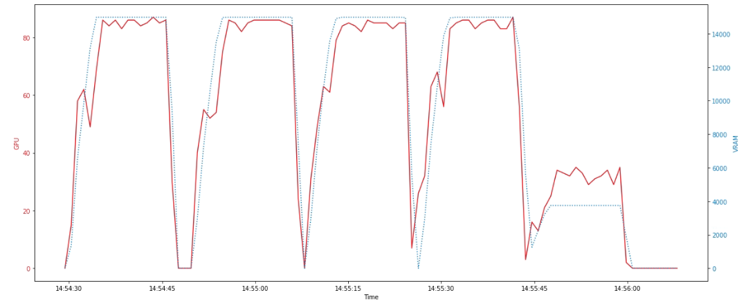
\includegraphics[width=0.8\textwidth]{images/experiment-lb-utilization-plot.png}
    \caption{GPU/VRAM Utilization Plot from \texttt{xgpg0\_2.log}}
    \label{fig:experiment-lb-utilization-plot}
\end{figure}

\section{Concurrency Experiment}
\label{s:concurrency-exp}
In this section, we will discuss the experiments about running multiple evaluation jobs \textbf{concurrently} on a \textbf{single} worker node. The objective is to show that our worker node can process multiple submissions in parallel with linear scalability.

Raw logs and analyzing scripts can be found in \href{https://github.com/edu-ai/aivle-experiment-logs}{aiVLE experiment logs repository}\footnote{\href{https://github.com/edu-ai/aivle-experiment-logs}{https://github.com/edu-ai/aivle-experiment-logs}}.For correspondence between experiment setup and log file index, please refer to Table~\ref{tab:concurrency-exp}

\begin{table}[H]
\centering
\begin{tabular}{|c|c|c|c|c|c|}
\hline
\multicolumn{1}{|l|}{\begin{tabular}[c]{@{}l@{}}Web\\ log index\end{tabular}} & \multicolumn{1}{l|}{\begin{tabular}[c]{@{}l@{}}Worker\\ log index\end{tabular}} & \multicolumn{1}{l|}{Node count} & \multicolumn{1}{l|}{\begin{tabular}[c]{@{}l@{}}Concurrency \\ of worker\end{tabular}} & \multicolumn{1}{l|}{Submission count} & \multicolumn{1}{l|}{\begin{tabular}[c]{@{}l@{}}Concurrency \\ of submission\end{tabular}} \\ \hline
7 & 4 & 1 & 8 & 100 & 100 \\ \hline
8 & 5 & 1 & 4 & 100 & 100 \\ \hline
9 & 6 & 1 & 2 & 100 & 100 \\ \hline
10 & 7 & 1 & 1 & 100 & 100 \\ \hline
\end{tabular}
\caption{Per-worker Concurrency Experiment Setup}
\label{tab:concurrency-exp}
\end{table}

\subsection{Methodology}
For explanation of parameters/variables, and the method of measuring total time please refer to Section~\ref{ss:lb-exp-meth}. For the per-worker concurrency experiment, we activate \textbf{only one} worker node, and measure \textbf{time taken} to finish 100 submissions with concurrency of worker ranging from 1, 2, 4 and 8.

\subsection{Results}

\begin{itemize}
    \item concurrency = 1: 1558.811s (baseline)
    \item concurrency = 2: 859.237s (90.71\%)
    \item concurrency = 4: 422.744s (92.18\%)
    \item concurrency = 8: 235.426s (82.77\%)
\end{itemize}

Similar to section \ref{ss:load-balancing-exp-results}, the percentage in the end is the scaling efficiency. The definition is also similar by changing the meaning of $N$ to the concurrency number.
